\begin{figure}[t]
\centering
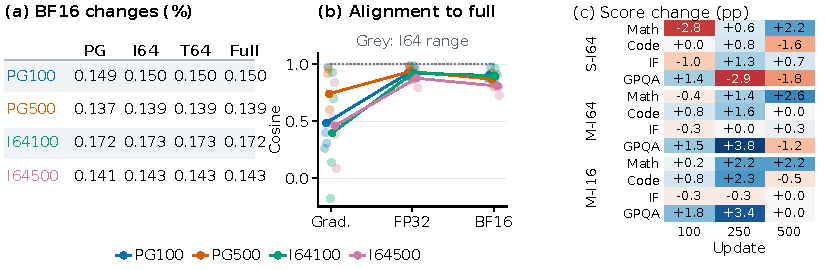
\includegraphics[width=\linewidth]{figures/table1_sync_20260918/section5_supervision.pdf}
\caption{\textbf{Top-64 supervision closely approximates the full-vocabulary gradient in Qwen and produces task-dependent learning gains.}
(a) Fraction of changed BF16 weights for each local loss at fixed checkpoints.
(b) Gradient and update cosines to full-vocabulary supervision.
(c) Score differences from sampled-token supervision over training. PG: sampled token; I16/I64: student--teacher top-16/top-64 intersection; T64: teacher top-64. S/M denote mathematics-only/joint training; checkpoint numbers are training updates.}
\label{fig:supervision_overview}
\end{figure}
